\documentclass[]{beamer}
\usepackage[T1]{fontenc}
\usepackage[utf8]{inputenc}
\usepackage{lmodern}
\usepackage[italian]{babel}
\usepackage{mathrsfs}

\title{La carica elettrica}
\author{\texorpdfstring{Mattia Cozzi\newline\href{mailto:cozzimattia@gmail.com}{\texttt{cozzimattia@gmail.com}}}{Mattia Cozzi}}
\date{a.s.~2023/2024}

%\documentclass[handout]{beamer}     %usare questa classe per generare l'handout
%\usepackage{pgfpages}   %per mostrare più quadri nella stessa pagina
%\pgfpagesuselayout{4 on 1}[a4paper,border shrink=5mm,landscape]
\usetheme{Singapore}
%\useoutertheme[left]{sidebar} %elementi intorno alle diapositive
\setbeamercovered{dynamic} %modifica l'aspetto del testo grigetto delle diapositive future. Argomenti: invisible/transparent/dynamic
\usecolortheme{orchid}
%COLORE PRINCIPALE
% \definecolor{marroncino}{RGB}{156, 26, 0} % UBC Blue (primary)
% \setbeamercolor{structure}{fg=marroncino} % itemize, enumerate, etc

\theoremstyle{plain}
\newtheorem{teorema}{Teorema}

\usepackage{tikz}
\usepackage{circuitikz}

\usepackage{pgf,pgfplots,graphicx}
\usetikzlibrary{angles,quotes,arrows,shapes,decorations.markings}
\pgfplotsset{compat=1.15}
\usepgfplotslibrary{units,fillbetween} % to add units easily to axis

\newcommand{\fem}{f_{em}}

\def\angolo[#1](#2)(#3:#4:#5)% Syntax: [draw options] (center) (initial angle:final angle:radius)
    { \draw[#1] ($(#2)+({#5*cos(#3)},{#5*sin(#3)})$) arc (#3:#4:#5); }


\begin{document}

\begin{frame}
  \titlepage
\end{frame}





\begin{frame}
\frametitle{Contenuti}
\tableofcontents
\end{frame}


\section{Modello}

\begin{frame}
  \frametitle{Corpi elettrizzati}
  \begin{columns}
    \begin{column}{0.3\textwidth}
      \begin{figure}
        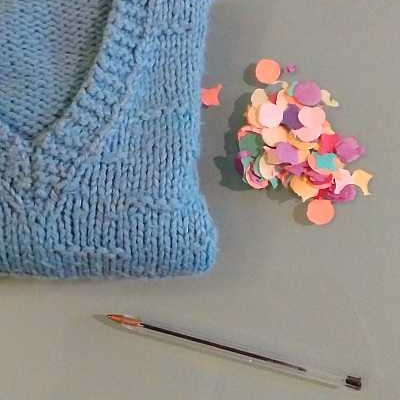
\includegraphics[width=\columnwidth]{img/maglione.jpg}
        
        Cosa succede sfregando la penna sul maglione?
      \end{figure}
    \end{column}
    \begin{column}{0.3\textwidth}
      \visible<2-3>{\begin{figure}
        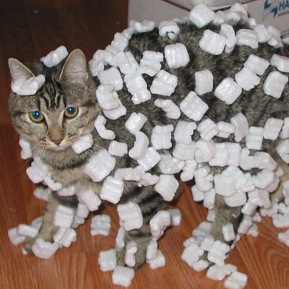
\includegraphics[width=\columnwidth]{img/gatto.jpg}
        
        Un gatto elettrizzato
        
        ~
      \end{figure}
      }
    \end{column}
    \begin{column}{0.3\textwidth}
      \visible<3>{\begin{figure}
        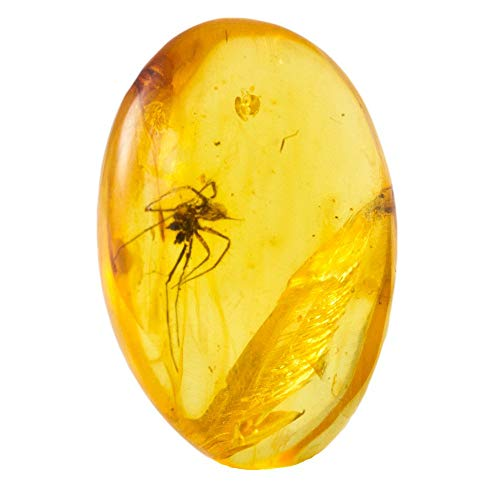
\includegraphics[width=\columnwidth]{img/ambra.jpg}
        
        $ \eta\lambda\varepsilon\kappa\tau\rho \textrm{\textit{o}} \nu $
        
        ~
        
        ~
      \end{figure}
      }
    \end{column}
  \end{columns}
\end{frame}


\begin{frame}
\frametitle{XVIII secolo}
\begin{columns}
\begin{column}{0.2\textwidth}
\visible<1->{\begin{figure}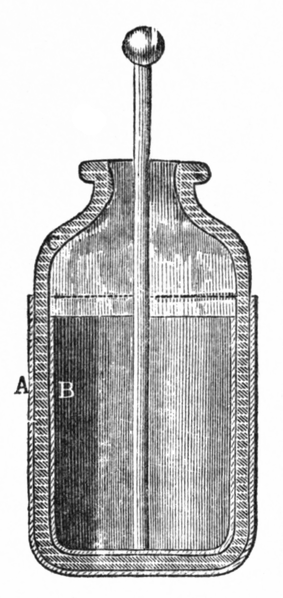
\includegraphics[width=.6\columnwidth]{img/leida.png}\end{figure}}
~
\visible<2->{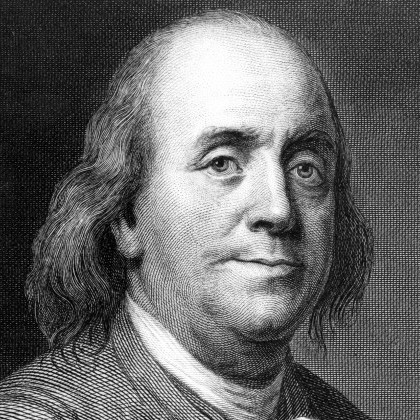
\includegraphics[width=\columnwidth]{img/franklin.jpg}}
\end{column}
\begin{column}{0.7\textwidth}
\begin{itemize}
\item<1-> Nel 1745 viene inventata la \alert<1>{bottiglia di Leida}, il primo dispositivo in grado di immagazzinare carica;\pause
\item<2-> nel 1747 Benjamin Franklin teorizza che gli oggetti siano elettrizzati in virtù di un eccesso (\alert<2>{carica positiva}) o un difetto (\alert<2>{carica negativa}) di un non meglio precisato ``fluido elettrico''.
\end{itemize}
\visible<3>{\alert{Corpi con cariche dello stesso segno si respingono, corpi con cariche opposte si attraggono.}}
\end{column}
\end{columns}
\end{frame}





\begin{frame}
\frametitle{Modello microscopico}
\begin{columns}
\begin{column}{0.2\textwidth}
\visible<2->{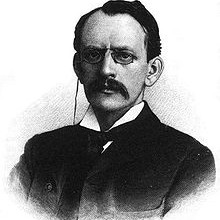
\includegraphics[width=\columnwidth]{img/thomson.jpg}}
~
\visible<3->{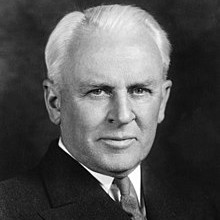
\includegraphics[width=\columnwidth]{img/millikan.jpg}}
~
\visible<4->{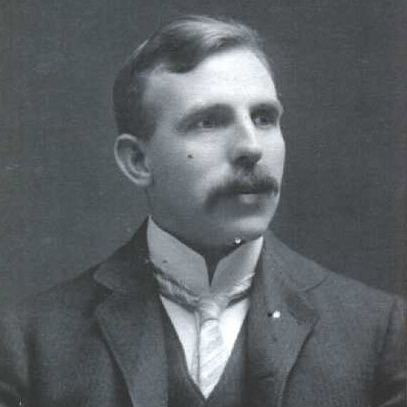
\includegraphics[width=\columnwidth]{img/rutherford.jpg}}
\end{column}
\begin{column}{0.7\textwidth}
Oggi sappiamo che la \alert<1>{carica di un corpo dipende dalla differenza tra il numero di protoni ($ p^{+} $) e quello di elettroni ($ e^{-} $)}.
\begin{itemize}
\item<2-> gli elettroni furono scoperti da Joseph J.~\alert<2>{Thomson} nel \alert<2>{1897};
\item<3-> la carica dell'elettrone fu misurata da Robert \alert<3>{Millikan} nel \alert<3>{1909};
\item<4-> il nucleo atomico fu scoperto da Ernest \alert<4->{Rutherford} nel \alert<4>{1911};
\item<5-> lo stesso Rutherford scopre il protone nel \alert<5>{1919}.
\end{itemize}
\end{column}
\end{columns}
\end{frame}


\begin{frame}
\frametitle{Elettroni}
\begin{figure}
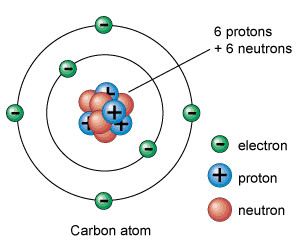
\includegraphics[width=.4\columnwidth]{img/atomino.jpg}
\end{figure}

Poiché i protoni sono vincolati tra loro nei nuclei atomici, in un corpo positivo avremo una carenza di elettroni, in uno negativo un eccesso di elettroni. 
\end{frame}



\section{Elettrizzazione (1)}


\begin{frame}
\frametitle{Isolanti e conduttori}
Distinguiamo due categorie di sostanze:
\begin{itemize}
  \item \alert<1>{isolanti}, cioè sostanze in cui le cariche non sono libere di muoversi;\pause
  \item \alert<2>{conduttori}, in cui le cariche (spesso elettroni) sono libere di muoversi.
\end{itemize}\pause~\\
\begin{alertblock}{Attenzione!}
  Vedremo più avanti che la distinzione tra isolanti e conduttori non è in realtà così netta, ma potremo stabilire diversi gradi di conduttività.
\end{alertblock}
\end{frame}






\begin{frame}
\frametitle{Elettrizzazione per strofinio}
\begin{figure}
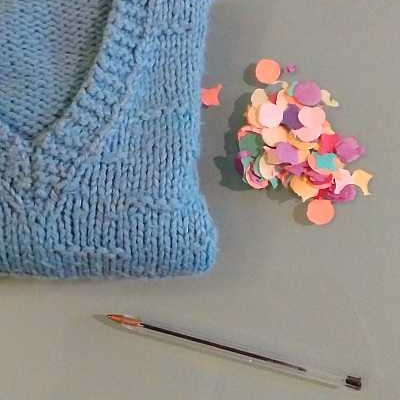
\includegraphics[width=.3\columnwidth]{img/maglione.jpg}
\end{figure}
Quando strofiniamo la penna sul maglione, \alert{spostiamo elettroni dal maglione alla penna}, che risulta carica negativamente. La carica viene poi dispersa a terra tramite il nostro corpo.\pause\\~\\

Si elettrizzano per strofinio gli isolanti oppure i conduttori isolati (impugnati ad esempio mediante un manico isolante).
\end{frame}



\begin{frame}
\frametitle{Elettrizzazione per contatto}
\begin{figure}
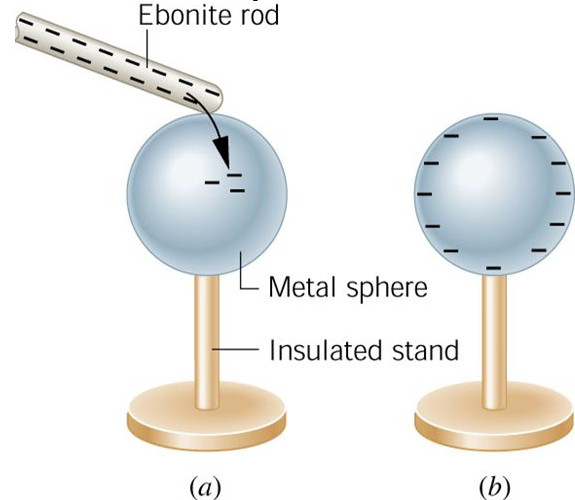
\includegraphics[width=.4\columnwidth]{img/contatto.jpg}
\end{figure}
Possiamo elettrizzare un conduttore isolato avvicinando ad esso un conduttore isolato caricato in precedenza.

Quando i conduttori si toccano, \alert{una parte della carica del secondo passa sul primo, caricandolo}.
\end{frame}





\begin{frame}
\frametitle{Elettroscopio}
\begin{columns}
\begin{column}{0.2\textwidth}
\visible<1->{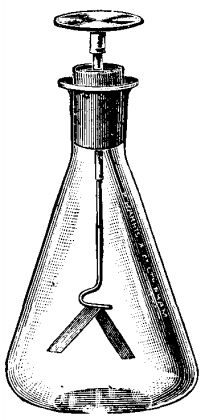
\includegraphics[width=\columnwidth]{img/elettroscopio.jpg}}
\end{column}
\begin{column}{0.7\textwidth}
L'elettrizzazione per contatto è sfruttata nell'elettroscopio, inventato nella sua forma moderna nel 1787, che permette di scoprire se un corpo è carico o meno.\pause

~

Quando tocchiamo la ``testa'' con un corpo carico, una parte della carica si distribuisce lungo l'asta e infine sulle foglioline d'oro, le quali \alert{si separano}.\pause

~

Non permette di scoprire il \emph{segno} della carica, ma può essere tarato per misurare la carica.
\end{column}
\end{columns}
\end{frame}



\section{Carica}

\begin{frame}
\frametitle{Carica elettrica}
Nel SI \alert<1>{la carica si misura in \emph{coulomb}}, simbolo $ C $.\pause

~

Poiché $ 1 \, C $ è una carica molto grande, spesso lavoreremo con i sottomultipli del \emph{coulomb}, in particolare:
\begin{itemize}
  \item $ 1 \, \mu C = 1 \times 10^{-6} \, C $
  \item $ 1 \, n C = 1 \times 10^{-9} \, C $
\end{itemize}\pause

~

Ogni elettrone (il \emph{quanto di carica elettrica}) ha una carica di:
\begin{center}
\colorbox{blue!30}{$ -e = - 1,6022 \times 10^{-19} \, C $}
\end{center}

Ogni carica elettrica è un multiplo (positivo o negativo) di $ e $.
\end{frame}


\begin{frame}
\frametitle{Elettroni e ioni}
Nel nostro studio incontreremo due tipi particelle cariche:
\begin{itemize}
  \item \alert<1>{elettroni}, di massa $ m_e = 9, 109 \times 10^{-31}  \, kg $ e carica $ -e $;\pause
  \item \alert<2>{ioni} (come $ Na^{+} $, $ Cl^{-} $ o $ Ca^{2+} $), atomi o molecole di massa variabile che hanno perso o guadagnato elettroni; $ Cl^{-} $ ha carica $ -e $, $ Ca^{2+} $ ha carica $ +2e $, ecc.
\end{itemize}
\visible<2>{
\begin{figure}
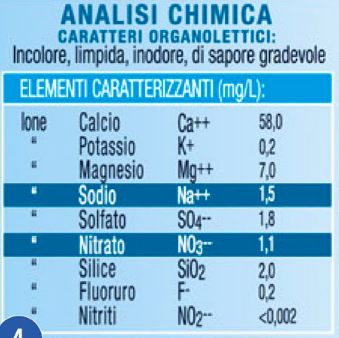
\includegraphics[width=.3\columnwidth]{img/etichetta.png}
\end{figure}
}
\end{frame}



\begin{frame}
\frametitle{Principio di conservazione}
\begin{block}{Principio di conservazione della carica elettrica}
In un sistema chiuso la somma algebrica delle cariche elettriche si mantiene
costante, qualunque siano i fenomeni che in esso hanno luogo.
\end{block}
\end{frame}

\section{Coulomb}


\begin{frame}
\frametitle{La legge di Coulomb (1)}
Nel 1785 Charles-Augustin de Coulomb, utilizzando una \emph{bilancia di torsione}, scopre una legge che permette di calcolare l'intensità della forza  tra due cariche.\pause

~

\begin{block}{Legge di Coulomb}
Due cariche $ q_1 $ e $ q_2 $, poste nel vuoto a distanza $ r $, esercitano l'una sull'altra una forza (attrattiva o repulsiva) di intensità:
\begin{center}
\colorbox{blue!30}{$ F = k_0 \,  \dfrac{q_1 \, q_2}{r^2} $}
\end{center}
$ k_0 = 8,99 \times 10^9 \, \frac{Nm^2}{C^2}$ =  costante elettrica del vuoto
\end{block}


\begin{center}
\href{video/Coulomb.mp4}{\beamergotobutton{Video: La bilancia di torsione}}
\end{center}
\end{frame}



\begin{frame}
\frametitle{La legge di Coulomb (2)}
\begin{figure}
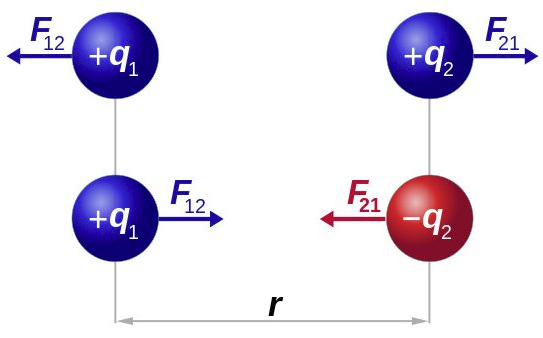
\includegraphics[width=.4\columnwidth]{img/leggecoulomb.png}
\end{figure}
Notiamo che la legge di Coulomb non fornisce direzione e verso della forza.{\pause} Essa avrà:
\begin{itemize}
  \item direzione lungo la retta che congiunge le cariche;\pause
  \item verso repulsivo per cariche dello stesso segno, attrattivo per cariche di segno opposto.
\end{itemize}
\end{frame}




\begin{frame}
\frametitle{Esempio 1}
\begin{exampleblock}{Intensità della forza}
{\small Due cariche di intensità $ - 3,2 \, \mu C $ e $ - 4,0 \, \mu C $ si trovano nel vuoto alla distanza di $ 7,0 \, cm $.
\begin{itemize}
  \item Rappresenta graficamente la situazione.
  \item Calcola l'intensità della forza agente tra le cariche.
\end{itemize}}
\end{exampleblock}\pause

~


\begin{center}
$ F =  \left( 8,99 \times 10^9 \, \dfrac{Nm^2}{C^2} \right) \dfrac{\left( 3,2 \times 10^{-6} \, C \right)\cdot\left( 4,0 \times 10^{-6} \, C \right)}{\left( 7,0 \times 10^{-2} \, m \right)^2} = $\pause

~

~

\visible<3>{$ = 2,3 \times 10^1 \, N = 23 \, N $}
\end{center}
\end{frame}




\begin{frame}
\frametitle{Esempio 2}
\begin{exampleblock}{Distanza tra le cariche}
{\small Due cariche di intensità $ 4,0 \, nC $ e $ 7,0 \, nC $ esercitano l'una sull'altra una forza di $ 5,3 \times 10^{-3} \, N $. Calcola la distanza tra le cariche.
}
\end{exampleblock}\pause

~

Invertiamo la formula della legge di Coulomb:
\begin{center}
$ F = k_0 \,  \dfrac{q_1 \, q_2}{r^2} ~~~\pause\Longrightarrow~~~ r^2 = k_0 \,  \dfrac{q_1 \, q_2}{F} ~~~\pause\Longrightarrow~~~ r = \sqrt{k_0 \,  \dfrac{q_1 \, q_2}{F}} $
\end{center}\pause
\begin{center}
$ r =  \sqrt{\left( 8,99 \times 10^9 \, \dfrac{Nm^2}{C^2} \right) \dfrac{\left( 4,0 \times 10^{-9} \, C \right)\cdot\left( 7,0 \times 10^{-9} \, C \right)}{5,3 \times 10^{-3} \, N}} = $
\end{center}\pause
\begin{center}
\visible<6>{$ = 6,9 \times 10^{-3} \, m $}
\end{center}
\end{frame}





\begin{frame}
\frametitle{Confronto con la forza di gravità}

\begin{columns}
\begin{column}{0.5\textwidth}
\begin{center}
\colorbox{blue!30}{$ F_C = k_0 \,  \dfrac{q_1 \, q_2}{r^2} $}

~

$ k_0 = 8,99 \times 10^9 \, \frac{Nm^2}{C^2}$
\end{center}
\visible<2->{Analogie:}
\begin{itemize}
  \item<2-> \alert<2>{stessa struttura};
  \item<3-> \alert<3>{agiscono a distanza};
  \item<4-> \alert<4>{direttamente prop.~ad una grandezza caratteristica};
  \item<5-> \alert<5>{inversamente prop.~al quadrato della distanza}.
\end{itemize}
\end{column}
\begin{column}{0.5\textwidth}
\begin{center}
\colorbox{blue!30}{$ F_N = G \,  \dfrac{m_1 \, m_2}{r^2} $}

~

$ G = 6,67 \times 10^{-11} \, \frac{Nm^2}{kg^2}$
\end{center}
\visible<6->{Differenze:}
\begin{itemize}
  \item<6-> \alert<6>{due tipi di carica, un tipo di massa};
  \item<7-> \alert<7>{$ F_C $ può essere attrattiva o repulsiva, $ F_N $ solo attrattiva};
  \item<8-> \alert<8>{$ F_C $ è, in condizioni ordinarie, molto più intensa di $ F_N $}.
\end{itemize}
\end{column}
\end{columns}
\end{frame}



\begin{frame}
\frametitle{Sovrapposizione}
Cosa succede quando una carica è sottoposta a più forze elettriche?\pause

~

\begin{block}{Principio di sovrapposizione}
La forza totale che agisce su una carica è uguale alla \alert{somma vettoriale} delle forze esercitate dalle singole cariche su di essa.
\end{block}
\visible<2>{\begin{figure}
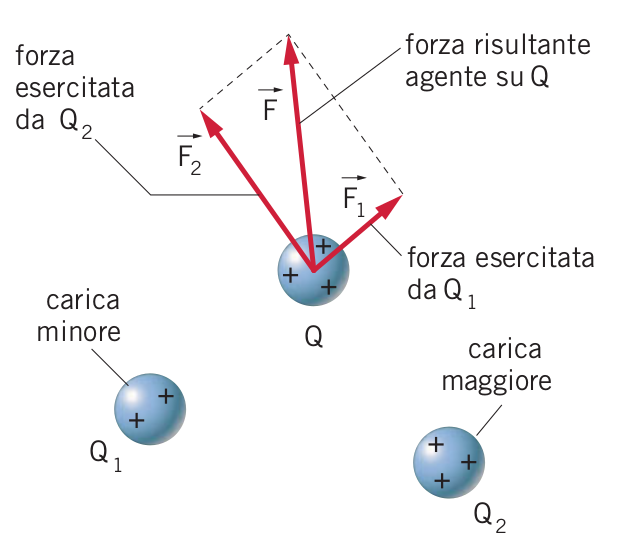
\includegraphics[width=.4\columnwidth]{img/sovrapposizionecariche.png}
\end{figure}}

\end{frame}



\begin{frame}
\frametitle{Esempio 3}
\begin{exampleblock}{Forza totale}
{\small Calcola l'intensità e il verso della forza totale agente su $ q_3 $.

\begin{figure}
\begin{tikzpicture}[scale=.5]
\draw (0,3) --(4,3);
\draw (9,3) --(4,3);
\node [above] at (6.5,3) {\footnotesize$ 4,5 \, mm $};
\node [above] at (2,3) {\footnotesize$ 4,0 \, mm $};
\draw [fill=blue] (0,3) circle [radius=0.1];
\node [below left] at (0,3) {\footnotesize $ q_1 = + 6,0 \, \mu C $};
\draw [fill=red] (4,3) circle [radius=0.1];
\node [below] at (4,3) {\footnotesize$ q_3 = - 3,0 \, \mu C $};
\draw [fill=blue] (9,3) circle [radius=0.1];
\node [below right] at (9,3) {\footnotesize$ q_2 = + 9,0 \, \mu C $};
\end{tikzpicture}
\end{figure}
}
\end{exampleblock}\pause


Rappresentiamo le forze agenti su $ q_3 $:
\begin{figure}
\begin{tikzpicture}[scale=.5]
\draw [thick,red,<-] (2,3) --(4,3);
\draw [thick,cyan,<-] (7,3) --(4,3);
\draw [fill=red] (4,3) circle [radius=0.1];
\node [below] at (4,3) {\footnotesize$ q_3 $};
\node [above,cyan] at (5.5,3) {\footnotesize$ F_2 $};
\node [above,red] at (3,3) {\footnotesize$ F_1 $};
\end{tikzpicture}\pause

~

$ F_{tot} = F_2 - F_1\pause = (1,2 \times 10^4 \, N) - (1,0 \times 10^4 \, N) =\pause 0,2 \times 10^4 \, N$

\end{figure}

\end{frame}




\begin{frame}
\frametitle{Esempio 4}
\begin{exampleblock}{Forza totale}
{\small Calcola intensità, direzione (rispetto all'orizzontale) e verso della forza totale agente su $ q_2 $.

\begin{figure}
\begin{tikzpicture}[scale=.5]
\draw (4,0) --(4,3);
\draw (0,3) --(4,3);
\node [right] at (4,1.5) {\footnotesize$ 6,0 \, mm $};
\node [above] at (2,3) {\footnotesize$ 8,0 \, mm $};
\draw [fill=blue] (0,3) circle [radius=0.1];
\node [above left] at (0,3) {\footnotesize $ q_1 = + 2,0 \, \mu C $};
\draw [fill=blue] (4,3) circle [radius=0.1];
\node [above right] at (4,3) {\footnotesize$ q_2 = + 1,0 \, \mu C $};
\draw [fill=blue] (4,0) circle [radius=0.1];
\node [below right] at (4,0) {\footnotesize$ q_3 = + 2,0 \, \mu C $};
\end{tikzpicture}
\end{figure}
}
\end{exampleblock}
\end{frame}


\begin{frame}
\frametitle{Esempio 4}
Rappresentiamo le forze agenti su $ q_2 $ e calcoliamo l'intensità delle due forze:

\begin{columns}
\begin{column}{0.3\textwidth}
\begin{figure}
\begin{tikzpicture}[scale=.5]
\draw[->,thick,red] (4,3) -- (4,6);
\draw[->,thick,cyan] (4,3) -- (6,3);
\node [below,cyan] at (5,3) {\footnotesize $ F_1 $};
\node [left,red] at (4,4.5) {\footnotesize $ F_3 $};
\draw[dashed] (4,0) --(4,3);
\node [right] at (4,1.5) {\footnotesize $ r_2 $};
\node [above] at (2,3) {\footnotesize $ r_1 $};
\draw[dashed] (0,3) --(4,3);
\draw [fill=blue] (0,3) circle [radius=0.1];
\node [above left] at (0,3) {\footnotesize $ q_1 $};
\draw [fill=blue] (4,3) circle [radius=0.1];
\node [above right] at (4,3) {\footnotesize$ q_2 $};
\draw [fill=blue] (4,0) circle [radius=0.1];
\node [below right] at (4,0) {\footnotesize$ q_3 $};
\end{tikzpicture}
\end{figure}
\end{column}
\begin{column}{0.6\textwidth}
\pause
\begin{center}
$ F_1 = k_0 \,  \dfrac{q_1 \, q_2}{r_1^2} = 2,8 \times 10^{2} \, N $

~\pause

~

$ F_3 = k_0 \,  \dfrac{q_3 \, q_2}{r_2^2} = 5,0 \times 10^{2} \, N $

~\pause

~

\colorbox{blue!30}{$ F_{tot} = (2,8)\hat{i} + (5,0)\hat{j} $}
\end{center}
\end{column}
\end{columns}

\end{frame}




\begin{frame}
\frametitle{Esempio 4}

Determiniamo l'intensità della forza totale con il TdP:
\begin{columns}
\begin{column}{0.3\textwidth}
\begin{figure}
\begin{tikzpicture}[scale=.9]
\angolo[teal,thick](4,3)(0:55:.6)
\node [above,teal] at (4.7,3.1) {\footnotesize$ \theta $};
\draw[dotted] (4,6) -- (6,6); 
\draw[dotted] (6,3) -- (6,6); 
\node [below left] at (4,3) {\footnotesize$ q_2 $};
\draw[->,thick,red!60] (4,3) -- (4,6);
\draw[->,thick,cyan!60] (4,3) -- (6,3);
\draw[->,thick,violet] (4,3) -- (6,6);
\node [below,cyan!60] at (5,3) {\footnotesize $ F_1 $};
\node [below right,violet] at (5,4.5) {\footnotesize $ F_{tot} $};
\node [left,red!60] at (4,4.5) {\footnotesize $ F_3 $};
\draw [fill=blue] (4,3) circle [radius=0.1];
\end{tikzpicture}
\end{figure}
\end{column}
\begin{column}{0.6\textwidth}
\begin{center}
$ F_{tot} = \sqrt{(F_1)^2 + (F_3)^2} = 5,7 \times 10^{2} \, N $
\end{center}
\end{column}
\end{columns}\pause
~

~

Per trovare l'angolo $ \theta $:
\begin{center}
$ \theta = \arcsin \left( \dfrac{F_3}{F_{tot}} \right) = \arccos \left( \dfrac{F_1}{F_{tot}} \right) = \arctan \left( \dfrac{F_3}{F_1} \right) = 61^{\circ} $
\end{center}
\end{frame}




\section{$ \varepsilon $}

\begin{frame}
\frametitle{La costante dielettrica del vuoto}
Per motivi che vedremo più avanti, si usa porre:
\begin{center}
$ k_0 = \dfrac{1}{4 \pi \varepsilon_0} $
\end{center}\pause
in cui compare la \alert{costante dielettrica del vuoto}:
\begin{center}
\colorbox{blue!30}{$ \varepsilon_0 = 8,854 \times 10^{-12} \,  \dfrac{C^2}{Nm^2} $}
\end{center}\pause
La legge di Coulomb sarà allora:
\begin{center}
$ F = \dfrac{1}{4 \pi \varepsilon_0} \,  \dfrac{q_1 \, q_2}{r^2} $
\end{center}
\end{frame}

\begin{frame}
\frametitle{La costante dielettrica relativa}
Si dimostra sperimentalmente che la forza elettrica tra due cariche ha il suo massimo valore nel vuoto.{\pause} Introduciamo allora la \alert{costante dielettrica relativa} di un mezzo:
\begin{center}
$ \varepsilon_r = \dfrac{F_{vuoto}}{F_{mezzo}} $~~~~~ovvero~~~~~$ F_{mezzo} = \dfrac{F_{vuoto}}{\varepsilon_r} $
\end{center}\pause

~

In un mezzo materiale la legge di Coulomb avrà la seguente forma:
\begin{center}
\colorbox{blue!30}{$ F = \dfrac{1}{4 \pi \varepsilon_0 \varepsilon_r} \,  \dfrac{q_1 \, q_2}{r^2} $}
\end{center}
\end{frame}





\begin{frame}
\frametitle{Valori della costante dielettrica relativa}
\centering
  \begin{tabular}{c|c}
    \textbf{Mezzo} & \textbf{$ \varepsilon_r $} \\\hline\rule{0pt}{3ex}
    Aria a $ 273 \, K $ & $ 1,00056 $ \\\rule{0pt}{3ex}
    Carta & $ 2,1 $ \\\rule{0pt}{3ex}
    Gomma & $ 2,3 $ \\\rule{0pt}{3ex}
    Vetro & $ 5-10 $ \\\rule{0pt}{3ex}
    Acqua & $ 80 $ \\
  \end{tabular}
\end{frame}






\section{Elettrizzazione (2)}


\begin{frame}
\frametitle{Elettrizzazione per induzione (1)}
Quando solleviamo un pezzetto di carta con una penna elettrizzata, stiamo attraendo un corpo scarico con uno carico. Come si spiega, data la legge di Coulomb?\pause
\visible<2>{
\begin{figure}
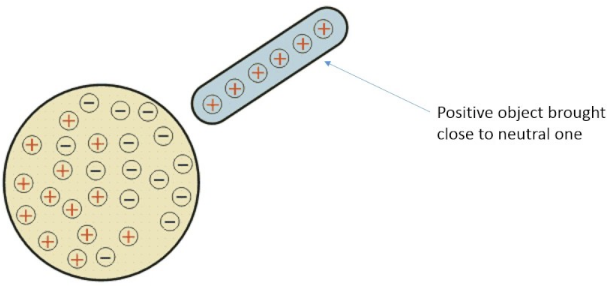
\includegraphics[width=.6\columnwidth]{img/induzione.png}
\end{figure}
}
Avviene una \alert{ridistribuzione delle cariche} all'interno del corpo scarico.

\end{frame}

\begin{frame}
\frametitle{Elettrizzazione per induzione (2)}
Se il corpo (globalmente neutro) viene collegato (messo) a terra, gli elettroni fluiscono nel suolo, lasciando il conduttore carico positivamente.
\begin{figure}
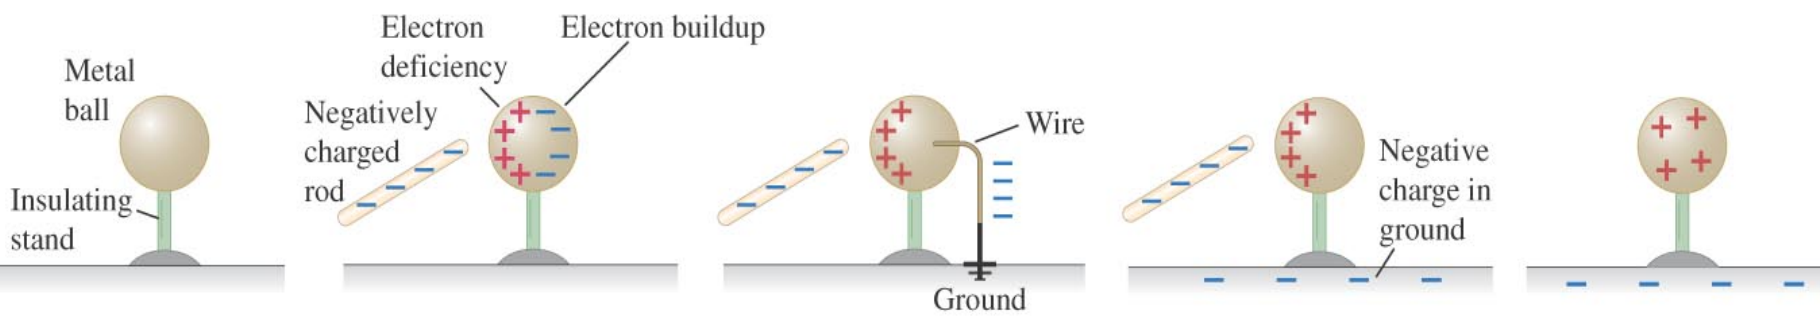
\includegraphics[width=\columnwidth]{img/induzione2.png}
\end{figure}
Vedere il \emph{riassunto sull'elettrizzazione} presente nel \underline{Formulario}.
\end{frame}



\begin{frame}
\frametitle{Polarizzazione}
In un isolante le cariche non sono libere di muoversi, ma possono orientarsi diversamente per la vicinanza di un corpo carico.
\begin{figure}
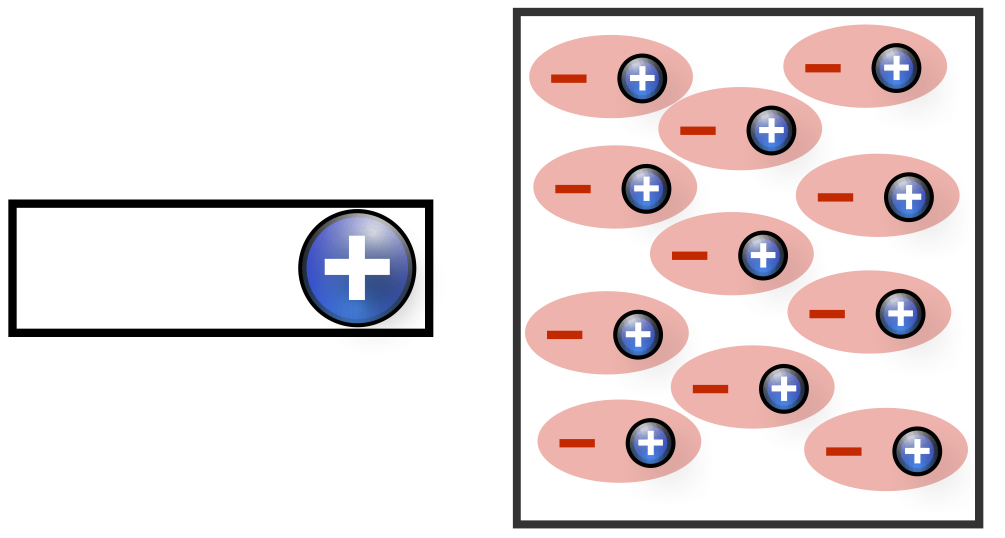
\includegraphics[width=.6\columnwidth]{img/polarizzazioneisolante.png}
\end{figure}
\end{frame}




\end{document}
